\chapter{Distribution of voice syncretism} \label{sect:distribution}
This chapter provides a distributional overview of voice syncretism in terms of type, frequency, and geography (\sectref{dist:syncretism}). For good measure, this overview also briefly covers the distribution of voices in general (\sectref{dist:voices}) as well as \isi{dedicated voice marking} (\sectref{dist:dedicated}) because voices are a prerequisite for voice syncretism, and voice marking which is not syncretic is per definition restricted to a single voice. The various statistics presented in this chapter are all based on the language sample of this book. The data underlying the statistics can be found in Appendices B and C. \tabref{tab:ch6:voice-syncretism} shows the number of languages (each represented by a WALS \isi{genus}) included in the language sample according to macroarea. The table also shows the number of languages in which at least one voice has been attested (+\textsc{v}) as well as the number of languages in which at least one pattern of voice syncretism has been attested (+\textsc{vs}). The first row of percentages is based on the numbers of genera\is{genus} in WALS according to macroarea (see \tabref{tab:ch1:wals} on page \pageref{tab:ch1:wals}) while the second and third rows of percentages are based on the genera\is{genus} included in this sample (see \tabref{tab:ch1:sample} on page \pageref{tab:ch1:sample}). As seen in the table, close to nine tenth of all the languages in the sample feature at least one voice (88.7 percent), while a little less than half of the languages in the sample feature at least one pattern of voice syncretism (46.8 percent).

\begin{table}
	\setlength{\tabcolsep}{2.2pt}
	\begin{tabularx}{\textwidth}{lrrrrrrrlrrrrrrrl}
		\lsptoprule
		& \multicolumn{1}{c}{\textbf{\textsc{af}}} & \multicolumn{1}{c}{\textbf{\textsc{ea}}} & \multicolumn{1}{c}{\textbf{\textsc{au}}} & \multicolumn{1}{c}{\textbf{\textsc{pn}}} & \multicolumn{1}{c}{\textbf{\textsc{na}}} & \multicolumn{1}{c}{\textbf{\textsc{sa}}} & \multicolumn{1}{c}{\textbf{Σ}} & & \multicolumn{1}{c}{\textbf{\textsc{af}}} & \multicolumn{1}{c}{\textbf{\textsc{ea}}} & \multicolumn{1}{c}{\textbf{\textsc{au}}} & \multicolumn{1}{c}{\textbf{\textsc{pn}}} & \multicolumn{1}{c}{\textbf{\textsc{na}}} & \multicolumn{1}{c}{\textbf{\textsc{sa}}} & \multicolumn{1}{c}{\textbf{Σ}} & \\
		\midrule
		\textbf{WALS} & 77 & 82 & 42 & 136 & 101 & 104 & 542 & & & & & & & & & \\
		\midrule
		\textbf{Sample} & 39 & 41 & 21 & 48 & 36 & 37 & 222 & (\#) & 50.6 & 50.0 & 50.0 & 35.3 & 35.6 & 35.6 & 41.0 & (\%) \\
		\multicolumn{1}{r}{\textbf{+\textsc{v}}} & 33 & 37 & 19 & 38 & 36 & 34 & 197 & & 84.6 & 90.2 & 90.5 & 79.2 & 100.0 & 91.9 & 88.7 & \\
		\multicolumn{1}{r}{\textbf{+\textsc{vs}}} & 19 & 20 & 14 & 9 & 19 & 23 & 104 & & 48.7 & 48.8 & 66.7 & 18.8 & 52.8 & 62.2 & 46.8 &\\
		\lspbottomrule
	\end{tabularx}
	\caption{Attestations of voice and voice syncretism in the sample}
	\label{tab:ch6:voice-syncretism}
\end{table} 

As \tabref{tab:ch6:voice-syncretism} shows, the percentual coverage of African, Eurasian, and Australian genera\is{genus} is higher than that of Papunesian, North American, and South American genera\is{genus} as a consequence of the \isi{bibliographical bias}. Nevertheless, as already discussed in \sectref{sample}, the proportional differences are not statistically significant, and the findings presented in this chapter are thus considered reasonably balanced and representative of the world’s languages. 

\section{Distribution of voices} \label{dist:voices}
The geographic distribution of languages with at least one voice in the sample is presented in \tabref{tab:ch6:voice-frequency}. The voices are listed according to their overall cross-linguistic frequency with the causative\is{causative voice} voice being most frequent and the antipassive\is{antipassive voice} voice being least frequent. Note that the anticausative\is{anticausative voice} and passive\is{passive voice} voices are equally frequent. As seen in the table, there is considerable variation in the prevalence of individual voices across the world, and voices are noticeably noticeably infrequent among languages of Papunesia. In fact, the Papunesian macroarea accounts for the lowest percentages of languages features causatives\is{causative voice}, reflexives\is{reflexive voice}, anticausatives\is{anticausative voice}, passives\is{passive voice}, and antipassives\is{antipassive voice}. By contrast, North America is characterised by a high prevalence of all seven voices. It is worth stressing here that this table and the other tables presented in this section say nothing about dissimilarities nor similarities in voice marking. Dissimilarities are briefly considered in terms of \isi{dedicated voice marking} in the next section, while similarities are discussed in more detail in terms of voice syncretism in \sectref{dist:syncretism}.

\begin{table}
	\setlength{\tabcolsep}{2.7pt}
	\begin{tabularx}{\textwidth}{lrrrrrrrlrrrrrrrl}
		\lsptoprule
		& \multicolumn{1}{c}{\textbf{\textsc{af}}} & \multicolumn{1}{c}{\textbf{\textsc{ea}}} & \multicolumn{1}{c}{\textbf{\textsc{au}}} & \multicolumn{1}{c}{\textbf{\textsc{pn}}} & \multicolumn{1}{c}{\textbf{\textsc{na}}} & \multicolumn{1}{c}{\textbf{\textsc{sa}}} & \multicolumn{1}{c}{\textbf{Σ}} & & \multicolumn{1}{c}{\textbf{\textsc{af}}} & \multicolumn{1}{c}{\textbf{\textsc{ea}}} & \multicolumn{1}{c}{\textbf{\textsc{au}}} & \multicolumn{1}{c}{\textbf{\textsc{pn}}} & \multicolumn{1}{c}{\textbf{\textsc{na}}} & \multicolumn{1}{c}{\textbf{\textsc{sa}}} & \multicolumn{1}{c}{\textbf{Σ}} & \\
		\midrule
		\textbf{\textsc{caus}} & 28 & 33 & 12 & 25 & 34 & 30 & 162 & (\#) & 71.8 & 80.5 & 57.1 & 52.1 & 94.4 & 81.1 & 73.9 & (\%) \\
		\textbf{\textsc{recp}} & 17 & 22 & 17 & 24 & 25 & 29 & 134 & & 43.6 & 53.7 & 81.0 & 50.0 & 69.4 & 78.4 & 60.4 & \\
		\textbf{\textsc{appl}} & 13 & 10 & 8 & 24 & 26 & 21 & 102 & & 33.3 & 24.4 & 38.1 & 50.0 & 72.2 & 56.8 & 45.9 & \\
		\textbf{\textsc{refl}} & 10 & 14 & 15 & 6 & 22 & 26 & 93 & & 25.6 & 34.1 & 71.4 & 12.5 & 61.1 & 70.3 & 41.9 & \\
		\textbf{\textsc{antc}} & 16 & 20 & 8 & 10 & 16 & 10 & 80 & & 41.0 & 48.8 & 38.1 & 20.8 & 44.4 & 27.0 & 36.0 & \\
		\textbf{\textsc{pass}} & 24 & 17 & 2 & 3 & 20 & 14 & 80 & & 61.5 & 41.5 & 9.5 & 6.3 & 55.6 & 37.8 & 36.0 & \\
		\textbf{\textsc{antp}} & 9 & 7 & 2 & 4 & 11 & 8 & 41 & & 23.1 & 17.1 & 9.5 & 8.3 & 30.6 & 21.6 & 18.5 & \\
		\midrule
		& & & & & & & & & \multicolumn{1}{c}{39} & \multicolumn{1}{c}{41} & \multicolumn{1}{c}{21} & \multicolumn{1}{c}{48} & \multicolumn{1}{c}{36} & \multicolumn{1}{c}{37} & \multicolumn{1}{c}{222} & (\textit{n}) \\
		\lspbottomrule
	\end{tabularx}
	\caption{Voices according to macroarea (by frequency)}
	\label{tab:ch6:voice-frequency}
\end{table} 

\tabref{tab:ch6:voice-macroarea} provides a different perspective on the geographic distribution of voices by showing the total number of voices (on the left-hand side of the table) attested in individual languages. Note that the maximum number of voices found in any given language is limited by the seven voices of focus in this book. The table shows that languages with three or four voices are most common in the language sample, while languages with seven voices are least common. Only eight languages of the latter kind are attested in the sample, five of which form two geographic clusters in the Americas: the Uto-Aztecan language Huasteca Nahuatl\il{Nahuatl, Huasteca}, the Totonacan language Filomeno Mata Totonac\il{Totonac, Filomeno Mata}, and the Oto-Manguean language Acazulco Otomí\il{Otomí, Acazulco} in the heart of Mexico; and the Panoan language \ili{Chácobo} and the isolate \ili{Mosetén} in Northwestern Bolivia. The remaining three languages are the Central Salish language \ili{Musqueam} of North America, the Kordofanian language \ili{Lumun} of Africa, and the language isolate \ili{Ainu} of Eurasia. Languages with seven voices are unattested in Australia and Papunesia. Only 25 languages in the sample (11.3 percent) feature no voice at all, none of which are spoken in North America. 

\begin{table}
	\setlength{\tabcolsep}{3pt}
	\begin{tabularx}{.97\textwidth}{clrrrrrrrlrrrrrrrl}
		\lsptoprule
		& & \multicolumn{1}{c}{\textbf{\textsc{af}}} & \multicolumn{1}{c}{\textbf{\textsc{ea}}} & \multicolumn{1}{c}{\textbf{\textsc{au}}} & \multicolumn{1}{c}{\textbf{\textsc{pn}}} & \multicolumn{1}{c}{\textbf{\textsc{na}}} & \multicolumn{1}{c}{\textbf{\textsc{sa}}} & \multicolumn{1}{c}{\textbf{Σ}} & & \multicolumn{1}{c}{\textbf{\textsc{af}}} & \multicolumn{1}{c}{\textbf{\textsc{ea}}} & \multicolumn{1}{c}{\textbf{\textsc{au}}} & \multicolumn{1}{c}{\textbf{\textsc{pn}}} & \multicolumn{1}{c}{\textbf{\textsc{na}}} & \multicolumn{1}{c}{\textbf{\textsc{sa}}} & \multicolumn{1}{c}{\textbf{Σ}} & \\
		\midrule
		\textbf{0} & & 6 & 4 & 2 & 10 & 0 & 3 & 25 & (\#) & 15.4 & 9.8 & 9.5 & 20.8 & 0.0 & 8.1 & 11.3 & (\%) \\
		\textbf{1} & & 3 & 9 & 1 & 9 & 3 & 1 & 26 & & 7.7 & 22.0 & 4.8 & 18.8 & 8.3 & 2.7 & 11.7 & \\
		\textbf{2} & & 7 & 2 & 6 & 12 & 3 & 6 & 36 & & 17.9 & 4.9 & 28.6 & 25.0 & 8.3 & 16.2 & 16.2 & \\
		\textbf{3} & & 7 & 8 & 4 & 9 & 6 & 5 & 39 & & 17.9 & 19.5 & 19.0 & 18.8 & 16.7 & 13.5 & 17.6 & \\
		\textbf{4} & & 6 & 10 & 2 & 5 & 7 & 8 & 38 & & 15.4 & 24.4 & 9.5 & 10.4 & 19.4 & 21.6 & 17.1 & \\
		\textbf{5} & & 6 & 3 & 5 & 2 & 7 & 8 & 31 & & 15.4 & 7.3 & 23.8 & 4.2 & 19.4 & 21.6 & 14.0 & \\
		\textbf{6} & & 3 & 4 & 1 & 1 & 6 & 4 & 19 & & 7.7 & 9.8 & 4.8 & 2.1 & 16.7 & 10.8 & 8.6 & \\
		\textbf{7} & & 1 & 1 & 0 & 0 & 4 & 2 & 8 & & 2.6 & 2.4 & 0.0 & 0.0 & 11.1 & 5.4 & 3.6 & \\
		\midrule
		& & & & & & & & & & \multicolumn{1}{c}{39} & \multicolumn{1}{c}{41} & \multicolumn{1}{c}{21} & \multicolumn{1}{c}{48} & \multicolumn{1}{c}{36} & \multicolumn{1}{c}{37} & \multicolumn{1}{c}{222} & (\textit{n}) \\
		\lspbottomrule
	\end{tabularx}
	\caption{Number of voices according to macroarea}
	\label{tab:ch6:voice-macroarea}
\end{table}

The percentages in \tabref{tab:ch6:voice-macroarea} are presented as cumulative percentages in \tabref{tab:ch6:voice-macroarea-cumulative}. The cumulative percentages for the Papunesian macroarea are consistently higher than those for other macroareas, while the cumulative percentages for the North American macroarea are consistently lower. For instance, 83.3 percent of Papunesian languages in the sample have three or fewer attested voices, while this is the case for only 33.3 percent of North American languages. Put differently, 66.7 percent of North American languages feature more than three voices, while the same number is only 16.7 percent for Papunesian languages. Languages of other macroareas lie somewhere in between these poles. 

\begin{table}
	\setlength{\tabcolsep}{3pt}
	\begin{tabularx}{.60\textwidth}{clrrrrrrl}
		\lsptoprule
		& & \multicolumn{1}{c}{\textbf{\textsc{af}}} & \multicolumn{1}{c}{\textbf{\textsc{ea}}} & \multicolumn{1}{c}{\textbf{\textsc{au}}} & \multicolumn{1}{c}{\textbf{\textsc{pn}}} & \multicolumn{1}{c}{\textbf{\textsc{na}}} & \multicolumn{1}{c}{\textbf{\textsc{sa}}} & \\
		\midrule
		\textbf{0} & & 15.4 & 9.8 & 9.5 & 20.8 & 0.0 & 8.1 & (\%) \\
		\textbf{1} & & 23.1 & 31.7 & 14.3 & 39.6 & 8.3 & 10.8 & \\
		\textbf{2} & & 41.0 & 36.6 & 42.9 & 64.6 & 16.7 & 27.0 & \\
		\textbf{3} & & 59.0 & 56.1 & 61.9 & 83.3 & 33.3 & 40.5 & \\
		\textbf{4} & & 74.4 & 80.5 & 71.4 & 93.8 & 52.8 & 62.2 & \\
		\textbf{5} & & 89.7 & 87.8 & 95.2 & 97.9 & 72.2 & 83.8 & \\
		\textbf{6} & & 97.4 & 97.6 & 100.0 & 100.0 & 88.9 & 94.6 & \\
		\textbf{7} & & 100.0 & 100.0 & 100.0 & 100.0 & 100.0 & 100.0 & \\
		\lspbottomrule
	\end{tabularx}
	\caption{Number of voices according to macroarea (cum.)}
	\label{tab:ch6:voice-macroarea-cumulative}
\end{table}

\newpage

Finally, \tabref{tab:ch6:voice-probability} shows the probability of any given language in the language sample with a particular voice (on the Y-axis) also having another voice (on the X-axis). For instance, if a language in the sample has a reflexive\is{reflexive voice} voice, the probability of it also featuring a reciprocal\is{reciprocal voice} voice is 94.6 percent. By contrast, if a language in the sample has a reciprocal\is{reciprocal voice} voice, the probability of it also featuring a reflexive\is{reflexive voice} voice is only 65.7 percent. The probabilities in this table are naturally closely linked to the overall frequencies of the respective voices (see \tabref{tab:ch6:voice-frequency} on page \pageref{tab:ch6:voice-frequency}), as reflected for instance by the consistently high probabilities of a language with a causative\is{causative voice} voice owing to the high prevalence of causative\is{causative voice} voices cross-linguistically. 

\begin{table}
	\setlength{\tabcolsep}{3pt}
	\begin{tabularx}{.78\textwidth}{llrrrrrrrl}
		\lsptoprule
		& & \multicolumn{1}{c}{\textbf{\textsc{refl}}} & \multicolumn{1}{c}{\textbf{\textsc{recp}}} & \multicolumn{1}{c}{\textbf{\textsc{antc}}} & \multicolumn{1}{c}{\textbf{\textsc{pass}}} & \multicolumn{1}{c}{\textbf{\textsc{antp}}} & \multicolumn{1}{c}{\textbf{\textsc{caus}}} &  \multicolumn{1}{c}{\textbf{\textsc{appl}}} & \\
		\midrule
		\textbf{\textsc{refl}} & → & \multicolumn{1}{c}{--} & 94.6 & 54.8 & 47.3 & 24.7 & 84.9 & 62.4 & (\%) \\
		\textbf{\textsc{recp}} & → & 65.7 & \multicolumn{1}{c}{--} & 44.8 & 43.3 & 19.4 & 82.8 & 60.4 & \\
		\textbf{\textsc{antc}} & → & 63.8 & 75.0 & \multicolumn{1}{c}{--} & 56.3 & 26.3 & 91.3 & 53.8 & \\
		\textbf{\textsc{pass}} & → & 55.0 & 72.5 & 56.3 & \multicolumn{1}{c}{--} & 28.8 & 92.5 & 50.0 & \\
		\textbf{\textsc{antp}} & → & 56.1 & 63.4 & 51.2 & 56.1 & \multicolumn{1}{c}{--} & 87.8 & 56.1 & \\
		\textbf{\textsc{caus}} & → & 48.8 & 68.5 & 45.1 & 45.7 & 22.2 & \multicolumn{1}{c}{--} & 53.7 & \\
		\textbf{\textsc{appl}} & → & 56.9 & 79.4 & 42.2 & 39.2 & 22.5 & 85.3 & \multicolumn{1}{c}{--} & \\
		\lspbottomrule
	\end{tabularx}
	\caption{Voices according to probability}
	\label{tab:ch6:voice-probability}
\end{table}

\section{Distribution of dedicated voice marking} \label{dist:dedicated}
As defined in Chapter \ref{voice-syncretism}, \isi{dedicated voice marking} refers to formal marking restricted to one of the seven voices of focus in this book. For example, in the Tupian language \ili{Karo} (\lang{sa}) the passive\is{passive voice} prefix \example{pe-}, the reflexive\is{reflexive voice} prefix \example{mãm-}, the reciprocal\is{reciprocal voice} prefix \example{ro-}, and the causative\is{causative voice} prefixes \example{ma-} and \example{ta-} are all regarded as \isi{dedicated voice marking} because the respective prefixes do not serve as voice marking in other voices \citep{gabas:1999}. The distribution of such \isi{dedicated voice marking} in the language sample is presented in \tabref{tab:ch6:voice-dedicated-1} according to macroarea. The table shows that a relatively low number of languages in the sample feature dedicated reflexive\is{reflexive voice}, anticausative\is{anticausative voice}, passive\is{passive voice}, or antipassive\is{antipassive voice} voice marking, while more than half of the languages feature dedicated causative\is{causative voice} voice marking. In turn, dedicated reciprocal\is{reciprocal voice} or applicative\is{applicative voice} voice marking is each attested in roughly one third of the languages in the sample. 

\begin{table}
	\setlength{\tabcolsep}{2.7pt}
	\begin{tabularx}{\textwidth}{lrrrrrrrlrrrrrrrl}
		\lsptoprule
		& \multicolumn{1}{c}{\textbf{\textsc{af}}} & \multicolumn{1}{c}{\textbf{\textsc{ea}}} & \multicolumn{1}{c}{\textbf{\textsc{au}}} & \multicolumn{1}{c}{\textbf{\textsc{pn}}} & \multicolumn{1}{c}{\textbf{\textsc{na}}} & \multicolumn{1}{c}{\textbf{\textsc{sa}}} & \multicolumn{1}{c}{\textbf{Σ}} & & \multicolumn{1}{c}{\textbf{\textsc{af}}} & \multicolumn{1}{c}{\textbf{\textsc{ea}}} & \multicolumn{1}{c}{\textbf{\textsc{au}}} & \multicolumn{1}{c}{\textbf{\textsc{pn}}} & \multicolumn{1}{c}{\textbf{\textsc{na}}} & \multicolumn{1}{c}{\textbf{\textsc{sa}}} & \multicolumn{1}{c}{\textbf{Σ}} & \\
		\midrule
		\textbf{\textsc{refl}} & 2 & 3 & 2 & 2 & 8 & 6 & 23 & (\#) & 5.1 & 7.3 & 9.5 & 4.2 & 22.2 & 16.2 & 10.4 & (\%) \\
		\textbf{\textsc{recp}} & 7 & 12 & 8 & 19 & 11 & 10 & 67 & & 17.9 & 29.3 & 38.1 & 39.6 & 30.6 & 27.0 & 30.2 & \\
		\textbf{\textsc{antc}} & 5 & 8 & 2 & 7 & 8 & 2 & 32 & & 12.8 & 19.5 & 9.5 & 14.6 & 22.2 & 5.4 & 14.4 & \\
		\textbf{\textsc{pass}} & 11 & 6 & 0 & 3 & 11 & 7 & 38 & & 28.2 & 14.6 & 0.0 & 6.3 & 30.6 & 18.9 & 17.1 & \\
		\textbf{\textsc{antp}} & 6 & 4 & 0 & 2 & 7 & 5 & 24 & & 15.4 & 9.8 & 0.0 & 4.2 & 19.4 & 13.5 & 10.8 & \\
		\textbf{\textsc{caus}} & 17 & 22 & 10 & 21 & 28 & 26 & 124 & & 43.6 & 53.7 & 47.6 & 43.8 & 77.8 & 70.3 & 55.9 & \\
		\textbf{\textsc{appl}} & 8 & 4 & 6 & 21 & 18 & 17 & 74 & & 20.5 & 9.8 & 28.6 & 43.8 & 50.0 & 45.9 & 33.3 & \\
		\midrule
		& & & & & & & & & \multicolumn{1}{c}{39} & \multicolumn{1}{c}{41} & \multicolumn{1}{c}{21} & \multicolumn{1}{c}{48} & \multicolumn{1}{c}{36} & \multicolumn{1}{c}{37} & \multicolumn{1}{c}{222} & (\textit{n}) \\
		\lspbottomrule
	\end{tabularx}
	\caption{Dedicated voice marking according to macroarea}
	\label{tab:ch6:voice-dedicated-1}
\end{table} 

\tabref{tab:ch6:voice-dedicated-2} provides a clearer picture of the relative proportions of \isi{dedicated voice marking}. This table is based on the same underlying figures as \tabref{tab:ch6:voice-dedicated-1} but the percentages are calculated according to the numbers of languages in the sample for which a given voice has been attested according to macroarea (see \tabref{tab:ch6:voice-frequency} on page \pageref{tab:ch6:voice-frequency}). For example, \tabref{tab:ch6:voice-dedicated-2} shows that in exactly half of the languages featuring a reciprocal\is{reciprocal voice} voice, this voice is characterised by dedicated reciprocal\is{reciprocal voice} marking. This percentage is considerably lower with regard to the reflexive\is{reflexive voice} voice, and considerably higher with regard to the causative\is{causative voice} and applicative\is{applicative voice} voices. As noted in the beginning of this chapter, \isi{dedicated voice marking} contrasts with voice syncretism, and the languages not covered by \tabref{tab:ch6:voice-dedicated-2} consequently feature voice syncretism. Thus, an inverse version of the table is provided and discussed in the next section (see \tabref{tab:ch6:voice-syncretism-macroarea-2} on page \pageref{tab:ch6:voice-syncretism-macroarea-2}). 

\begin{table}
	\setlength{\tabcolsep}{3pt}
	\begin{tabularx}{.64\textwidth}{lrrrrrrrl}
		\lsptoprule
		& \multicolumn{1}{c}{\textbf{\textsc{af}}} & \multicolumn{1}{c}{\textbf{\textsc{ea}}} & \multicolumn{1}{c}{\textbf{\textsc{au}}} & \multicolumn{1}{c}{\textbf{\textsc{pn}}} & \multicolumn{1}{c}{\textbf{\textsc{na}}} & \multicolumn{1}{c}{\textbf{\textsc{sa}}} & \multicolumn{1}{c}{\textbf{Σ}} & \\
		\midrule
		\textbf{\textsc{refl}} & 20.0 & 21.4 & 13.3 & 33.3 & 36.4 & 23.1 & 24.7 & (\%) \\
		\textbf{\textsc{recp}} & 41.2 & 54.5 & 47.1 & 79.2 & 44.0 & 34.5 & 50.0 & \\
		\textbf{\textsc{antc}} & 31.3 & 40.0 & 25.0 & 70.0 & 50.0 & 20.0 & 40.0 & \\
		\textbf{\textsc{pass}} & 45.8 & 35.3 & 0.0 & 100.0 & 55.0 & 50.0 & 47.0 & \\
		\textbf{\textsc{antp}} & 66.7 & 57.1 & 0.0 & 50.0 & 63.6 & 62.5 & 58.5 & \\
		\textbf{\textsc{caus}} & 60.7 & 66.7 & 83.3 & 84.0 & 82.4 & 86.7 & 76.5 & \\
		\textbf{\textsc{appl}} & 61.5 & 40.0 & 75.0 & 87.5 & 69.2 & 81.0 & 72.5 & \\
		\lspbottomrule
	\end{tabularx}
	\caption{Dedicated voice marking according to macroarea (prop.)}
	\label{tab:ch6:voice-dedicated-2}
\end{table}

\section{Distribution of voice syncretism} \label{dist:syncretism}
As shown in the beginning of this chapter, 104 of the 222 languages in the language sample (46.8 percent) feature voice syncretism (see \tabref{tab:ch6:voice-syncretism} on page \pageref{tab:ch6:voice-syncretism}). These languages are presented in \tabref{tab:ch6:voice-syncretism-type-1} according to type and macroarea. Type 1a syncretism denotes unconditioned full resemblance in voice marking\is{voice syncretism, full resemblance -- type 1} (\sectref{resemblance-type1a}), type 1b syncretism denotes conditioned full resemblance (\sectref{resemblance-type1b}), type 2 syncretism denotes partial resemblance\is{voice syncretism, partial resemblance -- type 2} (\sectref{resemblance-type2}), and type 3 syncretism denotes so-called reverse resemblance\is{voice syncretism, reverse resemblance -- type 3} (\sectref{resemblance-type3}). Note that a language can possess different types of voice syncretism for which reason it can be counted in several rows in the table. Moreover, note that the first row in the table denotes numbers of languages with type 1a and/or type 1b syncretism\is{voice syncretism, full resemblance -- type 1}. The numbers in this row happen to coincide with those for type 1a syncretism\is{voice syncretism, full resemblance -- type 1} in the following row, indicating that all languages in the sample featuring type 1b syncretism\is{voice syncretism, full resemblance -- type 1} also feature type 1a syncretism. \tabref{tab:ch6:voice-syncretism-type-1} shows that type 1 syncretism\is{voice syncretism, full resemblance -- type 1} is attested in 91 languages (41 percent), type 2 syncretism\is{voice syncretism, partial resemblance -- type 2} in 25 languages (11.3 percent), and type 3 syncretism\is{voice syncretism, reverse resemblance -- type 3} in six languages (2.7 percent). Observe that type 2 syncretism\is{voice syncretism, partial resemblance -- type 2} is not attested for a single Australian language in the sample, yet this type of syncretism is not entirely unknown to this macroarea as it has been attested in at least one Pama-Nyungan language in the literature, Uradhi (see \tabref{tab:ch1:nedjalkov-examples} on page \pageref{tab:ch1:nedjalkov-examples}).

\begin{table}
	\setlength{\tabcolsep}{2.8pt}
	\begin{tabularx}{\textwidth}{lrrrrrrrlrrrrrrrl}
		\lsptoprule
		& \multicolumn{1}{c}{\textbf{\textsc{af}}} & \multicolumn{1}{c}{\textbf{\textsc{ea}}} & \multicolumn{1}{c}{\textbf{\textsc{au}}} & \multicolumn{1}{c}{\textbf{\textsc{pn}}} & \multicolumn{1}{c}{\textbf{\textsc{na}}} & \multicolumn{1}{c}{\textbf{\textsc{sa}}} & \multicolumn{1}{c}{\textbf{Σ}} & & \multicolumn{1}{c}{\textbf{\textsc{af}}} & \multicolumn{1}{c}{\textbf{\textsc{ea}}} & \multicolumn{1}{c}{\textbf{\textsc{au}}} & \multicolumn{1}{c}{\textbf{\textsc{pn}}} & \multicolumn{1}{c}{\textbf{\textsc{na}}} & \multicolumn{1}{c}{\textbf{\textsc{sa}}} & \multicolumn{1}{c}{\textbf{Σ}} & \\
		\midrule
		\textbf{Type 1} & 15 & 19 & 14 & 6 & 17 & 20 & 91 & (\#) & 38.5 & 46.3 & 66.7 & 12.5 & 47.2 & 54.1 & 41.0 & (\%) \\
		\multicolumn{1}{r}{-- \textbf{a}} & 15 & 19 & 14 & 6 & 17 & 20 & 91 & & 38.5 & 46.3 & 66.7 & 12.5 & 47.2 & 54.1 & 41.0 & \\
		\multicolumn{1}{r}{-- \textbf{b}} & 3 & 0 & 0 & 0 & 3 & 0 & 6 & & 7.7 & 0.0 & 0.0 & 0.0 & 8.3 & 0.0 & 2.7 & \\
		\textbf{Type 2} & 4 & 5 & 0 & 3 & 3 & 10 & 25 & & 10.3 & 12.2 & 0.0 & 6.3 & 8.3 & 27.0 & 11.3 & \\
		\textbf{Type 3} & 0 & 2 & 1 & 1 & 0 & 2 & 6 & & 0.0 & 4.9 & 4.8 & 2.1 & 0.0 & 5.4 & 2.7 & \\
		\midrule
		& & & & & & & & & \multicolumn{1}{c}{39} & \multicolumn{1}{c}{41} & \multicolumn{1}{c}{21} & \multicolumn{1}{c}{48} & \multicolumn{1}{c}{36} & \multicolumn{1}{c}{37} & \multicolumn{1}{c}{222} & (\textit{n}) \\
		\lspbottomrule
	\end{tabularx}
	\caption{Voice syncretism according to type and macroarea}
	\label{tab:ch6:voice-syncretism-type-1}
\end{table} 

\newpage

\tabref{tab:ch6:voice-syncretism-type-2} is based on the same underlying numbers as \tabref{tab:ch6:voice-syncretism-type-1} but the percentages are calculated according to the numbers of languages for which voice syncretism has been attested in the sample. This table shows that close to nine tenth of the patterns of syncretism attested among the languages in the sample are of type 1\is{voice syncretism, full resemblance -- type 1} (87.5 percent), while roughly a quarter are of type 2\is{voice syncretism, partial resemblance -- type 2} (24.0 percent). Evidently, although type 2 syncretism\is{voice syncretism, partial resemblance -- type 2} has received little attention in the literature, it is not uncommon cross-linguistically.  Type 1\is{voice syncretism, full resemblance -- type 1} and type 2 syncretism\is{voice syncretism, partial resemblance -- type 2} serve as the basis for most of the statistics in the following sections, while type 3 syncretism\is{voice syncretism, reverse resemblance -- type 3} is largely ignored due to its peculiar nature (\sectref{resemblance-type3}), unless otherwise indicated. 

\begin{table}
	\setlength{\tabcolsep}{3pt}
	\begin{tabularx}{0.64\textwidth}{lrrrrrrrl}
		\lsptoprule
		& \multicolumn{1}{c}{\textbf{\textsc{af}}} & \multicolumn{1}{c}{\textbf{\textsc{ea}}} & \multicolumn{1}{c}{\textbf{\textsc{au}}} & \multicolumn{1}{c}{\textbf{\textsc{pn}}} & \multicolumn{1}{c}{\textbf{\textsc{na}}} & \multicolumn{1}{c}{\textbf{\textsc{sa}}} & \multicolumn{1}{c}{\textbf{Σ}} & \\
		\midrule
		\textbf{Type 1} & 78.9 & 95.0 & 100.0 & 66.7 & 89.5 & 87.0 & 87.5 & (\%) \\
		\multicolumn{1}{r}{-- \textbf{a}} & 78.9 & 95.0 & 100.0 & 66.7 & 89.5 & 87.0 & 87.5 & \\
		\multicolumn{1}{r}{-- \textbf{b}} & 15.8 & 0.0 & 0.0 & 0.0 & 15.8 & 0.0 & 5.8 & \\
		\textbf{Type 2} & 21.1 & 25.0 & 0.0 & 33.3 & 15.8 & 43.5 & 24.0 & \\
		\textbf{Type 3} & 0.0 & 10.0 & 7.1 & 11.1 & 0.0 & 8.7 & 5.8 & \\
		\midrule
		& \multicolumn{1}{c}{39} & \multicolumn{1}{c}{41} & \multicolumn{1}{c}{21} & \multicolumn{1}{c}{48} & \multicolumn{1}{c}{36} & \multicolumn{1}{c}{37} & \multicolumn{1}{c}{222} & (\textit{n}) \\
		\lspbottomrule
	\end{tabularx}
	\caption{Voice syncretism according to type and macroarea (prop.)}
	\label{tab:ch6:voice-syncretism-type-2}
\end{table} 

The geographic distribution of languages with voice syncretism in the language sample is presented in \tabref{tab:ch6:voice-syncretism-macroarea-1}. Observe that this table shows syncretic voice marking according to voice but does not show individual patterns of voice syncretism. For instance, the first cell in the table counts all African languages in which reflexive\is{reflexive voice} voice marking is syncretic with one voice or another. When the table is compared to the corresponding table on \isi{dedicated voice marking} in \sectref{dist:dedicated} (see \tabref{tab:ch6:voice-dedicated-1} on page \pageref{tab:ch6:voice-dedicated-1}), it is evident that more languages in the sample feature reflexive\is{reflexive voice}, anticausative\is{anticausative voice}, and/or passive\is{passive voice} syncretism than \isi{dedicated voice marking}. By contrast, more languages feature dedicated antipassive\is{antipassive voice}, causative\is{causative voice}, and/or applicative\is{applicative voice} \isi{dedicated voice marking} than voice syncretism. Interestingly, reciprocal\is{reciprocal voice} syncretism is equally prevalent as dedicated reciprocal\is{reciprocal voice} voice marking (30.2 percent), and the voice in question does therefore not seem to have any disposition towards neither dedicated marking nor syncretism.

\begin{table}
	\setlength{\tabcolsep}{2.7pt}
	\begin{tabularx}{.99\textwidth}{lrrrrrrrlrrrrrrrl}
		\lsptoprule
		& \multicolumn{1}{c}{\textbf{\textsc{af}}} & \multicolumn{1}{c}{\textbf{\textsc{ea}}} & \multicolumn{1}{c}{\textbf{\textsc{au}}} & \multicolumn{1}{c}{\textbf{\textsc{pn}}} & \multicolumn{1}{c}{\textbf{\textsc{na}}} & \multicolumn{1}{c}{\textbf{\textsc{sa}}} & \multicolumn{1}{c}{\textbf{Σ}} & & \multicolumn{1}{c}{\textbf{\textsc{af}}} & \multicolumn{1}{c}{\textbf{\textsc{ea}}} & \multicolumn{1}{c}{\textbf{\textsc{au}}} & \multicolumn{1}{c}{\textbf{\textsc{pn}}} & \multicolumn{1}{c}{\textbf{\textsc{na}}} & \multicolumn{1}{c}{\textbf{\textsc{sa}}} & \multicolumn{1}{c}{\textbf{Σ}} & \\
		\midrule
		\textbf{\textsc{refl}} & 8 & 11 & 13 & 4 & 14 & 20 & 70 & (\#) & 20.5 & 26.8 & 61.9 & 8.3 & 38.9 & 54.1 & 31.5 & (\%) \\
		\textbf{\textsc{recp}} & 10 & 10 & 9 & 5 & 14 & 19 & 67 & & 25.6 & 24.4 & 42.9 & 10.4 & 38.9 & 51.4 & 30.2 & \\
		\textbf{\textsc{antc}} & 11 & 12 & 6 & 3 & 8 & 8 & 48 & & 28.2 & 29.3 & 28.6 & 6.3 & 22.2 & 21.6 & 21.6 & \\
		\textbf{\textsc{pass}} & 13 & 11 & 2 & 0 & 9 & 7 & 42 & & 33.3 & 26.8 & 9.5 & 0.0 & 25.0 & 18.9 & 18.9 & \\
		\textbf{\textsc{antp}} & 3 & 3 & 2 & 2 & 4 & 3 & 17 & & 7.7 & 7.3 & 9.5 & 4.2 & 11.1 & 8.1 & 7.7 & \\
		\textbf{\textsc{caus}} & 11 & 11 & 2 & 4 & 6 & 4 & 38 & & 28.2 & 26.8 & 9.5 & 8.3 & 16.7 & 10.8 & 17.1 & \\
		\textbf{\textsc{appl}} & 5 & 6 & 2 & 3 & 8 & 4 & 28 & & 12.8 & 14.6 & 9.5 & 6.3 & 22.2 & 10.8 & 12.6 & \\
		\midrule
		& & & & & & & & & \multicolumn{1}{c}{39} & \multicolumn{1}{c}{41} & \multicolumn{1}{c}{21} & \multicolumn{1}{c}{48} & \multicolumn{1}{c}{36} & \multicolumn{1}{c}{37} & \multicolumn{1}{c}{222} & (\textit{n}) \\
		\lspbottomrule
	\end{tabularx}
	\caption{Voice syncretism according to macroarea}
	\label{tab:ch6:voice-syncretism-macroarea-1}
\end{table} 

\tabref{tab:ch6:voice-syncretism-macroarea-2} shows the proportions of the numbers in \tabref{tab:ch6:voice-syncretism-macroarea-1} in relation to the numbers of languages in the sample for which a given voice is attested according to macroarea (see \tabref{tab:ch6:voice-frequency} on page \pageref{tab:ch6:voice-frequency}). Thus, \tabref{tab:ch6:voice-syncretism-macroarea-2} is basically an inverse version of the corresponding table on \isi{dedicated voice marking} presented in \sectref{dist:dedicated} (see \tabref{tab:ch6:voice-dedicated-2} on page \pageref{tab:ch6:voice-dedicated-2}). \tabref{tab:ch6:voice-syncretism-macroarea-2} shows that voice marking in the reflexive\is{reflexive voice} voice is predominantly syncretic, while the voice marking in causative\is{causative voice} and applicative\is{applicative voice} voices is predominantly dedicated. Voice marking in the remaining voices lie in between these poles. The cross-linguistic prevalence of reflexive\is{reflexive voice} syncretism is particularly interesting in relation to the fact that reflexivity\is{reflexive voice} is commonly the centre of attention in studies of voice syncretism (\sectref{middle-voice}). The high overall percentage clearly shows that reflexive\is{reflexive voice} voice marking is more prone to be syncretic than voice marking associated with other voices, and the traditional focus on reflexive\is{reflexive voice} syncretism is therefore not unfounded. Furthermore, it can be observed that passive\is{passive voice} voice marking is consistently dedicated among Papunesian languages but syncretic among Australian languages. Likewise, antipassive\is{antipassive voice} voice marking is consistently syncretic for the latter languages. However, it is worth keeping in mind that the passive\is{passive voice} and antipassive\is{antipassive voice} voices are rather uncommon among languages of these two macroareas in the first place. 

\begin{table}
	\setlength{\tabcolsep}{3pt}
	\begin{tabularx}{.63\textwidth}{lrrrrrrrl}
		\lsptoprule
		& \multicolumn{1}{c}{\textbf{\textsc{af}}} & \multicolumn{1}{c}{\textbf{\textsc{ea}}} & \multicolumn{1}{c}{\textbf{\textsc{au}}} & \multicolumn{1}{c}{\textbf{\textsc{pn}}} & \multicolumn{1}{c}{\textbf{\textsc{na}}} & \multicolumn{1}{c}{\textbf{\textsc{sa}}} & \multicolumn{1}{c}{\textbf{Σ}} & \\
		\midrule
		\textbf{\textsc{refl}} & 80.0 & 78.6 & 86.7 & 66.7 & 63.6 & 76.9 & 75.3 & (\%) \\
		\textbf{\textsc{recp}} & 58.8 & 45.5 & 52.9 & 20.8 & 56.0 & 65.5 & 50.0 & \\
		\textbf{\textsc{antc}} & 68.8 & 60.0 & 75.0 & 30.0 & 50.0 & 80.0 & 60.0 & \\
		\textbf{\textsc{pass}} & 54.2 & 64.7 & 100.0 & 0.0 & 45.0 & 50.0 & 52.5 & \\
		\textbf{\textsc{antp}} & 33.3 & 42.9 & 100.0 & 50.0 & 36.4 & 37.5 & 41.5 & \\
		\textbf{\textsc{caus}} & 39.3 & 33.3 & 16.7 & 16.0 & 17.6 & 13.3 & 23.5 & \\
		\textbf{\textsc{appl}} & 38.5 & 60.0 & 25.0 & 12.5 & 30.8 & 19.0 & 27.5 & \\
		\lspbottomrule
	\end{tabularx}
	\caption{Voice syncretism according to macroarea (prop.)}
	\label{tab:ch6:voice-syncretism-macroarea-2}
\end{table}

Next, \tabref{tab:ch6:voice-syncretism-complexity} provides a more detailed overview of the numbers of individual voices that share voice marking. The Y-axis denotes a given voice and its voice marking, while the X-axis indicates the number of other voices sharing the same voice marking. For example, the table shows that 39.8 percent of reflexive\is{reflexive voice} voice syncretism attested in the sample involves the reflexive\is{reflexive voice} voice in addition to one other voice. By contrast, only 1.1 percent of the attestations involves the reflexive\is{reflexive voice} voice in addition to four other voices. The table also covers \isi{dedicated voice marking} (“0”) for easy reference and comparison, while the final column in the table (“2–4”) represents the cumulative percentages of the three previous columns. For instance, the latter column shows that voice marking in the anticausative\is{anticausative voice} voice is more likely to be shared by two or more voices (35 percent) than just one other voice (25 percent). The same goes for voice marking in the antipassive\is{antipassive voice} voice (cf. 29.3 percent and 12.1 percent, respectively). By contrast, the opposite is true for voice marking in the other voices. This shows that that anticausative\is{anticausative voice} and antipassive\is{antipassive voice} voices are more commonly linked with multiple other voices in terms of voice marking than the reflexive\is{reflexive voice}, reciprocal\is{reciprocal voice}, causative\is{causative voice}, and applicative\is{applicative voice} voices. This can probably be explained to some extent by the fact that the anticausative\is{anticausative voice} and antipassive\is{antipassive voice} voices are more likely to evolve from other voices than to serve as origins of voice syncretism themselves, as further discussed in the next chapter. Furthermore, it can be observed that causative\is{causative voice} or applicative\is{applicative voice} voice marking only rarely is shared by more than one other voice. The most notable exception here is the North Omotic language \ili{Wolaytta} (\lang{af}), which features causative-passive-reflexive-reciprocal syncretism (\sectref{sec:complex-syncretism:caus-pass}). Additionally, note that the Permic language Udmurt (\lang{ea}) is the only language featured in the column “4” due to its extensive syncretism (\sectref{sec:complex-syncretism:multiplex}). 

\begin{table}
	\setlength{\tabcolsep}{2.7pt}
	\begin{tabularx}{.77\textwidth}{lrrrrrlrrrrrrl}
		\lsptoprule
		& \multicolumn{1}{c}{\textbf{0}} & \multicolumn{1}{c}{\textbf{1}} & \multicolumn{1}{c}{\textbf{2}} & \multicolumn{1}{c}{\textbf{3}} & \multicolumn{1}{c}{\textbf{4}} & & \multicolumn{1}{c}{\textbf{0}} & \multicolumn{1}{c}{\textbf{1}} & \multicolumn{1}{c}{\textbf{2}} & \multicolumn{1}{c}{\textbf{3}} & \multicolumn{1}{c}{\textbf{4}} & \multicolumn{1}{c}{\textbf{2--4}} & \\
		\midrule
		\textbf{\textsc{refl}} & 23 & 37 & 25 & 7 & 1 & (\#) & 24.7 & 39.8 & 26.9 & 7.5 & 1.1 & 35.5 & (\%) \\
		\textbf{\textsc{recp}} & 67 & 34 & 26 & 6 & 1 & & 50.0 & 25.4 & 19.4 & 4.5 & 0.7 & 24.6 & \\
		\textbf{\textsc{antc}} & 32 & 20 & 21 & 6 & 1 & & 40.0 & 25.0 & 26.3 & 7.5 & 1.3 & 35.0 & \\
		\textbf{\textsc{pass}} & 38 & 22 & 15 & 4 & 1 & & 47.5 & 27.5 & 18.8 & 5.0 & 1.3 & 25.0 & \\
		\textbf{\textsc{antp}} & 24 & 5 & 7 & 4 & 1 & & 58.5 & 12.2 & 17.1 & 9.8 & 2.4 & 29.3 & \\
		\textbf{\textsc{caus}} & 124 & 32 & 5 & 1 & 0 & & 76.5 & 19.8 & 3.1 & 0.6 & 0.0 & 3.7 & \\
		\textbf{\textsc{appl}} & 74 & 24 & 4 & 0 & 0 & & 72.5 & 23.5 & 3.9 & 0.0 & 0.0 & 3.9 & \\
		\lspbottomrule
	\end{tabularx}
	\caption{Voice syncretism according to complexity}
	\label{tab:ch6:voice-syncretism-complexity}
\end{table} 

A more detailed discussion of the distribution of the patterns of simplex voice syncretism\is{voice syncretism, simplex} underlying the figures in column “1” is provided in the next section, while the patterns of complex voice syncretism\is{voice syncretism, complex} underlying the figures in columns “2” through “4” are treated in more detail in \sectref{dist:maximal}.

\subsection{By minimal syncretism} \label{dist:minimal} % dist:simplex
\tabref{tab:ch6:voice-syncretism-simplex} shows the distribution of minimal\is{voice syncretism, minimal} simplex voice syncretism\is{voice syncretism, simplex} in the language sample according to pattern and type. Thus, here the attestation of, say, reflexive-reciprocal-anticausative syncretism in a language is counted under the patterns “\textsc{refl-recp}”, “\textsc{refl-recp}” and “\textsc{recp-antc}”. Maximal\is{voice syncretism, maximal} simplex\is{voice syncretism, simplex} and complex syncretism\is{voice syncretism, complex} (excluding minimal\is{voice syncretism, minimal} syncretism) is treated separately in the next section. The 21 patterns listed in the table are sorted according to frequency (type 1\is{voice syncretism, full resemblance -- type 1} and type 2 syncretism\is{voice syncretism, partial resemblance -- type 2} combined) with the most frequent pattern at the top and the least frequent pattern at the bottom. Furthermore, note that the attestations of type 1\is{voice syncretism, full resemblance -- type 1} and type 2\is{voice syncretism, partial resemblance -- type 2} presented in \tabref{tab:ch6:voice-syncretism-simplex} do not necessarily sum up to the combined figures horizontally, as some languages feature both types and are therefore only counted once in the sums. Also note that the attestations of type 3 syncretism\is{voice syncretism, reverse resemblance -- type 3} do not sum up to six vertically in the table, even though it was mentioned in \sectref{resemblance-type3} that the phenomenon is attested in six languages in the sample. This is due to the fact that more than one pattern of type 3 voice syncretism\is{voice syncretism, reverse resemblance -- type 3} is attested in both the language isolate \ili{Mosetén} (\lang{sa}) and the Gunwinyguan language \ili{Nunggubuyu} (\lang{au}). Moreover, observe that no pattern of simplex voice syncretism\is{voice syncretism, simplex} is attested in more than one fourth of the language sample, and that all but two patterns are attested in less than ten percent. Evidently, most patterns of simplex voice syncretism\is{voice syncretism, simplex} are not particularly common cross-linguistically. However, it is worth keeping in mind that each language in the sample represents a unique \isi{genus}, many of which encompass multiple other languages. Thus, it is predicted that there are hundreds of additional languages around the world featuring one or more of the patterns in \tabref{tab:ch6:voice-syncretism-simplex}.

\begin{table}
	\setlength{\tabcolsep}{3.4pt}
	\begin{tabularx}{\textwidth}{lrrrrrrlrrrrrrl}
		\lsptoprule
		& \multicolumn{1}{c}{\textbf{1a+b}} & \multicolumn{1}{c}{\textbf{1a}} & \multicolumn{1}{c}{\textbf{1b}} & \multicolumn{1}{c}{\textbf{2}} & \multicolumn{1}{c}{\textbf{3}} & \multicolumn{1}{c}{\textbf{1+2}} & & \multicolumn{1}{c}{\textbf{1a+b}} & \multicolumn{1}{c}{\textbf{1a}} & \multicolumn{1}{c}{\textbf{1b}} & \multicolumn{1}{c}{\textbf{2}} & \multicolumn{1}{c}{\textbf{3}} & \multicolumn{1}{c}{\textbf{1+2}} & \\
		\midrule
		\textbf{\textsc{refl-recp}} & 43 & 43 & 0 & 8 & 0 & 49 & (\#) & 19.4 & 19.4 & 0.0 & 3.6 & 0.0 & 22.1 & (\%) \\
		\textbf{\textsc{refl-antc}} & 33 & 32 & 1 & 0 & 0 & 33 & & 14.9 & 14.4 & 0.5 & 0.0 & 0.0 & 14.9 & \\
		\textbf{\textsc{recp-antc}} & 18 & 17 & 1 & 4 & 0 & 22 & & 8.1 & 7.7 & 0.5 & 1.8 & 0.0 & 9.9 & \\
		\textbf{\textsc{caus-appl}} & 18 & 17 & 1 & 2 & 2 & 20 & & 8.1 & 7.7 & 0.5 & 0.9 & 0.9 & 9.0 & \\
		\textbf{\textsc{pass-refl}} & 17 & 17 & 0 & 2 & 0 & 19 & & 7.7 & 7.7 & 0.0 & 0.9 & 0.0 & 8.6 & \\
		\textbf{\textsc{pass-antc}} & 17 & 17 & 0 & 0 & 0 & 17 & & 7.7 & 7.7 & 0.0 & 0.0 & 0.0 & 7.7 & \\
		\textbf{\textsc{pass-recp}} & 9 & 9 & 0 & 6 & 0 & 15 & & 4.1 & 4.1 & 0.0 & 2.7 & 0.0 & 6.8 & \\
		\textbf{\textsc{caus-pass}} & 9 & 7 & 2 & 5 & 0 & 14 & & 4.1 & 3.2 & 0.9 & 2.3 & 0.0 & 6.3 & \\
		\textbf{\textsc{antp-recp}} & 11 & 11 & 0 & 0 & 0 & 11 & & 5.0 & 5.0 & 0.0 & 0.0 & 0.0 & 5.0 & \\
		\textbf{\textsc{antp-refl}} & 10 & 10 & 0 & 0 & 0 & 10 & & 4.5 & 4.5 & 0.0 & 0.0 & 0.0 & 4.5 & \\
		\textbf{\textsc{antp-antc}} & 10 & 9 & 1 & 0 & 0 & 10 & & 4.5 & 4.1 & 0.5 & 0.0 & 0.0 & 4.5 & \\
		\textbf{\textsc{appl-recp}} & 3 & 3 & 0 & 5 & 3 & 8 & & 1.4 & 1.4 & 0.0 & 2.3 & 1.4 & 3.6 & \\
		\textbf{\textsc{caus-antc}} & 4 & 3 & 1 & 1 & 0 & 5 & & 1.8 & 1.4 & 0.5 & 0.5 & 0.0 & 2.3 & \\
		\textbf{\textsc{pass-antp}} & 4 & 4 & 0 & 0 & 0 & 4 & & 1.8 & 1.8 & 0.0 & 0.0 & 0.0 & 1.8 & \\
		\textbf{\textsc{caus-recp}} & 2 & 1 & 1 & 2 & 1 & 4 & & 0.9 & 0.5 & 0.5 & 0.9 & 0.5 & 1.8 & \\
		\textbf{\textsc{appl-pass}} & 2 & 2 & 0 & 1 & 1 & 3 & & 0.9 & 0.9 & 0.0 & 0.5 & 0.5 & 1.4 & \\
		\textbf{\textsc{appl-antp}} & 2 & 2 & 0 & 0 & 1 & 2 & & 0.9 & 0.9 & 0.0 & 0.0 & 0.5 & 0.9 & \\
		\textbf{\textsc{caus-antp}} & 2 & 1 & 1 & 0 & 0 & 2 & & 0.9 & 0.5 & 0.5 & 0.0 & 0.0 & 0.9 & \\
		\textbf{\textsc{caus-refl}} & 1 & 0 & 1 & 1 & 0 & 2 & & 0.5 & 0.0 & 0.5 & 0.5 & 0.0 & 0.9 & \\
		\textbf{\textsc{appl-refl}} & 0 & 0 & 0 & 1 & 2 & 1 & & 0.0 & 0.0 & 0.0 & 0.5 & 0.9 & 0.5 & \\
		\textbf{\textsc{appl-antc}} & 0 & 0 & 0 & 0 & 0 & 0 & & 0.0 & 0.0 & 0.0 & 0.0 & 0.0 & 0.0 & \\
		\lspbottomrule
	\end{tabularx}
	\caption{Minimal voice syncretism according to type}
	\label{tab:ch6:voice-syncretism-simplex}
\end{table} 

\tabref{tab:ch6:voice-syncretism-simplex} shows that patterns of \isi{middle syncretism} are generally much more frequent cross-linguistically than other patterns with the notable exception of causative-applicative syncretism. It is, however, also worth noting that three patterns of antipassive\is{antipassive voice} syncretism are attested in ten to eleven genera\is{genus}, and also that causative-passive syncretism is roughly as common as passive-reciprocal syncretism. All other patterns are rather uncommon and two remain unattested as type 1\is{voice syncretism, full resemblance -- type 1} syncretism, applicative-reflexive and applicative-anticausative syncretism. As already discussed in \sectref{geniusiene-syncretism} and \sectref{haspelmath-syncretism}, patterns of simplex \isi{middle syncretism}\is{voice syncretism, simplex} have also been found to be cross-linguistically more prevalent than other patterns of simplex voice syncretism\is{voice syncretism, simplex} in prior typological studies implicitly involving voice syncretism by \citet{geniusiene:1987} and \citet{haspelmath:1990}. Explicit comments on the cross-lingusitic prevalence of \isi{middle syncretism} can also be found sporadically in the literature. For example, as already cited in \sectref{sec:simple-syncretism:refl-recp}, \citet[66]{creissels:2016} argues that “[t]he reflexive-reciprocal syncretism does not seem to be particularly widespread in the languages of the world”. \citet[430]{maslova:nedjalkov:2005}, on the contrary, argue that in every fourth language “[t]he reciprocal\is{reciprocal voice} and reflexive\is{reflexive voice} constructions are formally identical”, and \citet[171]{heine:miyashita:2008} that “at least every third language has a \textsc{ref[l]-rec[p]} category”. Nevertheless, it is here worth noting that the estimates by \citeauthor{maslova:nedjalkov:2005} and \citeauthor{heine:miyashita:2008} also include periphrastic constructions of various kinds, unlike in this book. In any case, their estimates are rather close to the figures 19.4 percent (type 1 syncretism\is{voice syncretism, full resemblance -- type 1}) and 22.1 percent (type 1 and type 2 syncretism\is{voice syncretism, partial resemblance -- type 2} combined) attested in the survey of this book.

Sporadic comments on the cross-linguistic prevalence of other common patterns of voice syncretism can also be found in the literature, for instance on causative-applicative syncretism. \citet[116]{shibatani:pardeshi:2002} state that “[i]n a fair number of languages, causative\is{causative voice} morphemes are associated with the applicative\is{applicative voice} function”, and \citet[182]{peterson:2007} remarks that “[c]ausative-applicative syncretism is something which is not reported very frequently for causative\is{causative voice} markers explicitly, but it does occur”. \citet[10]{malchukov:2017} argues that the syncretism in question “seems actually to be more widespread cross-linguistically than reported”. Indeed, \tabref{tab:ch6:voice-syncretism-simplex} shows that causative-applicative syncretism is more prevalent than several patterns of \isi{middle syncretism}. By contrast, observations on the prevalence of less frequent patterns of syncretism are very scarce. One observation is provided by \citet[10]{creissels:2012} who remarks that passive-antipassive syncretism (alongside various other patterns of syncretism) “are extremely common cross-linguistically”. By contrast, \citet[151]{dixon:1994} states that “[j]ust occasionally, one finds a language in which a single derivational\is{derivation} affix can have either passive or antipassive\is{antipassive voice} effect”, and \citet[241]{zuniga:kittila:2019} argues that passive-antipassive syncretism is “rather difficult to find”. These suspicions can be confirmed here, as the syncretism is only attested in four languages in the sample. \citet[244]{zuniga:kittila:2019} also remark that they have only found “one clear case” of causative-anticausative syncretism, yet the sample this pattern of syncretism has roughly the same frequency as passive-antipassive syncretism. 

\begin{table}[b]
	\setlength{\tabcolsep}{3.2pt}
	\begin{tabularx}{\textwidth}{lrrrrrrlrrrrrrl}
		\lsptoprule
		& \multicolumn{1}{c}{\textbf{\textsc{af}}} & \multicolumn{1}{c}{\textbf{\textsc{ea}}} & \multicolumn{1}{c}{\textbf{\textsc{au}}} & \multicolumn{1}{c}{\textbf{\textsc{pn}}} & \multicolumn{1}{c}{\textbf{\textsc{na}}} & \multicolumn{1}{c}{\textbf{\textsc{sa}}} & & \multicolumn{1}{c}{\textbf{\textsc{af}}} & \multicolumn{1}{c}{\textbf{\textsc{ea}}} & \multicolumn{1}{c}{\textbf{\textsc{au}}} & \multicolumn{1}{c}{\textbf{\textsc{pn}}} & \multicolumn{1}{c}{\textbf{\textsc{na}}} & \multicolumn{1}{c}{\textbf{\textsc{sa}}} & \\
		\midrule
		\textbf{\textsc{refl-recp}} & 3 & 6 & 9 & 2 & 10 & 13 & (\#) & 7.7 & 14.6 & 42.9 & 4.2 & 27.8 & 35.1 & (\%) \\
		\textbf{\textsc{refl-antc}} & 4 & 8 & 6 & 3 & 6 & 6 & & 10.3 & 19.5 & 28.6 & 6.3 & 16.7 & 16.2 & \\
		\textbf{\textsc{recp-antc}} & 3 & 5 & 2 & 1 & 5 & 2 & & 7.7 & 12.2 & 9.5 & 2.1 & 13.9 & 5.4 & \\
		\textbf{\textsc{caus-appl}} & 3 & 4 & 2 & 2 & 5 & 2 & & 7.7 & 9.8 & 9.5 & 4.2 & 13.9 & 5.4 & \\
		\textbf{\textsc{pass-refl}} & 4 & 4 & 2 & 0 & 2 & 5 & & 10.3 & 9.8 & 9.5 & 0.0 & 5.6 & 13.5 & \\
		\textbf{\textsc{pass-antc}} & 5 & 6 & 1 & 0 & 3 & 2 & & 12.8 & 14.6 & 4.8 & 0.0 & 8.3 & 5.4 & \\
		\textbf{\textsc{pass-recp}} & 3 & 3 & 0 & 0 & 1 & 2 & & 7.7 & 7.3 & 0.0 & 0.0 & 2.8 & 5.4 & \\
		\textbf{\textsc{caus-pass}} & 3 & 3 & 0 & 0 & 3 & 0 & & 7.3 & 7.3 & 0.0 & 0.0 & 8.3 & 0.0 & \\
		\textbf{\textsc{antp-recp}} & 1 & 3 & 2 & 0 & 3 & 2 & & 2.6 & 7.3 & 9.5 & 0.0 & 8.3 & 5.4 & \\
		\textbf{\textsc{antp-refl}} & 0 & 3 & 2 & 1 & 2 & 2 & & 0.0 & 7.3 & 9.5 & 2.1 & 5.6 & 5.4 & \\
		\textbf{\textsc{antp-antc}} & 1 & 3 & 1 & 1 & 2 & 2 & & 2.6 & 7.3 & 4.8 & 2.1 & 5.6 & 5.4 & \\
		\textbf{\textsc{appl-recp}} & 1 & 0 & 0 & 0 & 2 & 0 & & 2.6 & 0.0 & 0.0 & 0.0 & 5.6 & 0.0 & \\
		\textbf{\textsc{caus-antc}} & 0 & 3 & 0 & 0 & 1 & 0 & & 0.0 & 7.3 & 0.0 & 0.0 & 2.8 & 0.0 & \\
		\textbf{\textsc{pass-antp}} & 0 & 2 & 0 & 0 & 1 & 1 & & 0.0 & 4.9 & 0.0 & 0.0 & 2.8 & 2.7 & \\
		\textbf{\textsc{caus-recp}} & 1 & 0 & 0 & 0 & 0 & 1 & & 2.6 & 0.0 & 0.0 & 0.0 & 0.0 & 2.7 & \\
		\textbf{\textsc{appl-pass}} & 0 & 1 & 0 & 0 & 1 & 0 & & 0.0 & 2.4 & 0.0 & 0.0 & 2.8 & 0.0 & \\
		\textbf{\textsc{appl-antp}} & 0 & 1 & 0 & 0 & 1 & 0 & & 0.0 & 2.4 & 0.0 & 0.0 & 2.8 & 0.0 & \\
		\textbf{\textsc{caus-antp}} & 1 & 0 & 0 & 1 & 0 & 0 & & 2.6 & 0.0 & 0.0 & 2.1 & 0.0 & 0.0 & \\
		\textbf{\textsc{caus-refl}} & 1 & 0 & 0 & 0 & 0 & 0 & & 2.6 & 0.0 & 0.0 & 0.0 & 0.0 & 0.0 & \\
		\textbf{\textsc{appl-refl}} & 0 & 0 & 0 & 0 & 0 & 0 & & 0.0 & 0.0 & 0.0 & 0.0 & 0.0 & 0.0 & \\
		\textbf{\textsc{appl-antc}} & 0 & 0 & 0 & 0 & 0 & 0 & & 0.0 & 0.0 & 0.0 & 0.0 & 0.0 & 0.0 & \\
		\lspbottomrule
	\end{tabularx}
	\caption{Minimal simplex voice syncretism (type 1)}
	\label{tab:ch6:voice-syncretism-macroarea-minimal}
\end{table}

Next, \tabref{tab:ch6:voice-syncretism-macroarea-minimal} shows the distribution of simplex voice syncretism\is{voice syncretism, simplex} according to macroarea\is{macroarea}. The order in which the patterns are listed in the table follows that of \tabref{tab:ch6:voice-syncretism-simplex} discussed above. However, note that \tabref{tab:ch6:voice-syncretism-macroarea-minimal} only covers type 1 syncretism\is{voice syncretism, full resemblance -- type 1} for which reason both applicative-reflexive and applicative-anticausative syncretism is unattested in the table. The table shows that are are considerable differences in the prevalence of voice syncretism across the world. Voice syncretism is noticeably more rare in Papunesia than in other macroareas\is{macroarea}, and only seven patterns of voice syncretism have been attested in the area. Only nine patterns of voice syncretism have been attested in Australia, yet in this area there is a high prevalence of reflexive-reciprocal and reflexive-anticausative syncretism. Indeed, the prevalence of reflexive-reciprocal syncretism in Australia is not matched by any other macroarea\is{macroarea}. By contrast, more than ten patterns of voice syncretism have been attested in each of the remaining four macroareas\is{macroarea}. North America is home to most diversity in voice syncretism with sixteen different patterns attested, followed by Eurasia with fifteen, Africa with fourteen, and South America with twelve. Only five patterns have been attested in all six macroareas\is{macroarea}: reflexive-reciprocal, reflexive-anticausative, reciprocal-anticausative, causative-applicative, and antipassive-anticausative syncretism. However, it is worth noting that three additional patterns have been attested in five macroareas\is{macroarea} each and the lack of attestations from a sixth macroarea\is{macroarea} can very well be coincidental: passive-reflexive, passive-anticausative, and antipassive-reciprocal syncretism. All other patterns of voice syncretism only show up sporadically and remain unattested or marginally attested in most macroareas\is{macroarea}.  

\begin{table}[b]
	\setlength{\tabcolsep}{3pt}
	\begin{tabularx}{.79\textwidth}{llrrrrrrrl}
		\lsptoprule
		& & \multicolumn{1}{c}{\textbf{\textsc{refl}}} & \multicolumn{1}{c}{\textbf{\textsc{recp}}} & \multicolumn{1}{c}{\textbf{\textsc{antc}}} & \multicolumn{1}{c}{\textbf{\textsc{pass}}} & \multicolumn{1}{c}{\textbf{\textsc{antp}}} & \multicolumn{1}{c}{\textbf{\textsc{caus}}} &  \multicolumn{1}{c}{\textbf{\textsc{appl}}} & \\
		\midrule
		\textbf{\textsc{refl}} & → & \multicolumn{1}{c}{--} & 52.7 & 35.5 & 20.5 & 10.8 & 2.2 & 1.1 & (\%) \\
		\textbf{\textsc{recp}} & → & 36.6 & \multicolumn{1}{c}{--} & 16.4 & 11.2 & 8.2 & 3.0 & 6.0 & \\
		\textbf{\textsc{antc}} & → & 41.3 & 27.5 & \multicolumn{1}{c}{--} & 21.3 & 12.5 & 6.3 & 0.0 & \\
		\textbf{\textsc{pass}} & → & 23.8 & 18.8 & 21.3 & \multicolumn{1}{c}{--} & 5.0 & 17.5 & 3.8 & \\
		\textbf{\textsc{antp}} & → & 24.4 & 26.8 & 24.4 & 9.8 & \multicolumn{1}{c}{--} & 4.9 & 4.9 & \\
		\textbf{\textsc{caus}} & → & 1.2 & 2.5 & 3.1 & 8.6 & 1.2 & \multicolumn{1}{c}{--} & 12.3 & \\
		\textbf{\textsc{appl}} & → & 1.0 & 7.8 & 0.0 & 2.9 & 2.0 & 19.6 & \multicolumn{1}{c}{--} & \\
		\lspbottomrule
	\end{tabularx}
	\caption{Voice syncretism according to probability}
	\label{tab:ch6:voice-syncretism-probability}
\end{table}

Finally, \tabref{tab:ch6:voice-syncretism-probability} shows the probability of voice marking in a particular voice (on the Y-axis) being syncretic with voice marking in another voice (on the X-axis) among the languages in the language sample. For instance, if a language in the sample has a reflexive\is{reflexive voice} voice, the probability of its reflexive\is{reflexive voice} voice marking being syncretic with reciprocal\is{reciprocal voice} voice marking is 52.7 percent. In other words, a reflexive\is{reflexive voice} voice is attested in 93 languages in the sample (see \tabref{tab:ch6:voice-frequency} on page \pageref{tab:ch6:voice-frequency}) and 49 of the aforementioned languages (52.7 percent) feature reflexive-reciprocal syncretism (see \tabref{tab:ch6:voice-syncretism-simplex}). By contrast, if a language has an applicative\is{applicative voice} voice, the probability of its applicative\is{applicative voice} voice marking being syncretic with anticausative\is{anticausative voice} voice marking is zero percent, as no such pattern of voice syncretism is attested at all. In light of the data presented and discussed in this and the previous section, it is not surprising that the probabilities for patterns of \isi{middle syncretism} are generally higher than those for other patterns in \tabref{tab:ch6:voice-syncretism-probability}. However, it is also worth noting the comparatively high probabilities pertaining to causative\is{causative voice} and applicative\is{applicative voice} voice marking which highlights the close relationship between the two voices seen in many languages (\sectref{sec:simple-syncretism:caus-appl}). Indeed, as discussed in more detail in the next chapter, it appears that causative\is{causative voice} voice marking can develop an applicative\is{applicative voice} function (\sectref{diachrony:caus2appl}) and applicative\is{applicative voice} voice marking can develop a causative\is{causative voice} function (\sectref{diachrony:appl2caus}). Likewise, observe the comparatively high probability of passive\is{passive voice} voice marking being syncretic with causative\is{causative voice} voice marking (i.e. 17.5 percent). Causative\is{causative voice} voice marking is known to have developed a passive\is{passive voice} function in a variety of languages (\sectref{diachrony:caus2pass}).

\subsection{By maximal syncretism} \label{dist:maximal} % dist:complex
\tabref{tab:ch6:voice-syncretism-maximal-simplex-macroarea} shows the distribution of maximal\is{voice syncretism, maximal} simplex voice syncretism\is{voice syncretism, simplex} in the language sample according to macroarea\is{macroarea}. Thus, unlike in the previous section, the table only encompasses voice marking restricted to two voices (e.g. \ili{Rotokas} reflexive-reciprocal marking \example{ora-} with no other voice functions). Moreover, the figures in the table represent type 1 attestations\is{voice syncretism, full resemblance -- type 1} though type 2 attestations\is{voice syncretism, partial resemblance -- type 2} are provided for comparison at the right hand side. The various patterns in the table are listed according to the type 1 attestations\is{voice syncretism, full resemblance -- type 1} with the most frequent pattern in the top and the least frequent patterns at the bottom. The order of the patterns in this table is evidently very different from that discussed in the previous section. For instance, voice marking shared by the reciprocal\is{reciprocal voice} and anticausative\is{anticausative voice} voices (minimal\is{voice syncretism, minimal} syncretism) is very common cross-linguistically (see \tabref{tab:ch6:voice-syncretism-macroarea-minimal} on page \pageref{tab:ch6:voice-syncretism-macroarea-minimal}) yet is very often also shared by one or two other voices, while voice marking restricted specifically to the reciprocal\is{reciprocal voice} and anticausative\is{anticausative voice} voices alone (maximal\is{voice syncretism, maximal} syncretism) has so far only been attested in a single language (see \tabref{tab:ch6:voice-syncretism-maximal-simplex-macroarea}). By contrast, reflexive-reciprocal syncretism is the most common pattern in terms of both minimal\is{voice syncretism, minimal} and maximal syncretism\is{voice syncretism, maximal}. Reflexive-reciprocal syncretism is one of three patterns of maximal syncretism\is{voice syncretism, maximal} in \tabref{tab:ch6:voice-syncretism-maximal-simplex-macroarea} attested in each of the six macroareas\is{macroarea}, the other two patterns being causative-applicative and reflexive-anticausative syncretism. These are also the only three patterns that are moderately common cross-linguistically. Other patterns of maximal voice syncretism\is{voice syncretism, maximal} are quite rare and are generally only attested in three macroareas\is{macroarea} or less. In fact, as seen at the bottom of the table, four patterns remain unattested as type 1 syncretism\is{voice syncretism, full resemblance -- type 1} altogether, while five other patterns are marginally attested in one language each.

\begin{sidewaystable}
	\setlength{\tabcolsep}{4.8pt}
	\begin{tabularx}{\textwidth}{lrrrrrrrlrrrrrrrlrrr}
		\lsptoprule
		& \multicolumn{1}{c}{\textbf{\textsc{af}}} & \multicolumn{1}{c}{\textbf{\textsc{ea}}} & \multicolumn{1}{c}{\textbf{\textsc{au}}} & \multicolumn{1}{c}{\textbf{\textsc{pn}}} & \multicolumn{1}{c}{\textbf{\textsc{na}}} & \multicolumn{1}{c}{\textbf{\textsc{sa}}} & \multicolumn{1}{c}{\textbf{Sum}} & & \multicolumn{1}{c}{\textbf{\textsc{af}}} & \multicolumn{1}{c}{\textbf{\textsc{ea}}} & \multicolumn{1}{c}{\textbf{\textsc{au}}} & \multicolumn{1}{c}{\textbf{\textsc{pn}}} & \multicolumn{1}{c}{\textbf{\textsc{na}}} & \multicolumn{1}{c}{\textbf{\textsc{sa}}} & \multicolumn{1}{c}{\textbf{Sum}} & & cf. & \multicolumn{2}{l}{\textbf{Type 2}} \\
		\midrule
		\textbf{\textsc{refl-recp}} & 1 & 2 & 7 & 1 & 5 & 8 & 24 & (\#) & 2.6 & 4.9 & 33.3 & 2.1 & 13.9 & 21.6 & 10.8 & (\%) & & 7 & (3.2 \%) \\
		\textbf{\textsc{caus-appl}} & 3 & 3 & 2 & 2 & 4 & 2 & 16 & & 7.7 & 7.3 & 9.5 & 4.2 & 11.1 & 5.4 & 7.2 & & & 2 & (0.9 \%) \\
		\textbf{\textsc{refl-antc}} & 2 & 3 & 2 & 1 & 1 & 4 & 13 & & 5.1 & 7.3 & 9.5 & 2.1 & 2.8 & 10.8 & 5.9 & & & 0 & (0.0 \%) \\
		\textbf{\textsc{pass-antc}} & 3 & 2 & 0 & 0 & 2 & 0 & 7 & & 7.7 & 4.9 & 0.0 & 0.0 & 5.6 & 0.0 & 3.2 & & & 0 & (0.0 \%) \\
		\textbf{\textsc{caus-pass}} & 2 & 2 & 0 & 0 & 2 & 0 & 6 & & 5.1 & 4.9 & 0.0 & 0.0 & 5.6 & 0.0 & 2.7 & & & 5 & (2.3 \%) \\
		\textbf{\textsc{pass-refl}} & 2 & 0 & 1 & 0 & 1 & 2 & 6 & & 5.1 & 0.0 & 4.8 & 0.0 & 2.8 & 5.4 & 2.7 & & & 2 & (0.9 \%) \\
		\textbf{\textsc{caus-antc}} & 0 & 2 & 0 & 0 & 1 & 0 & 3 & & 0.0 & 4.9 & 0.0 & 0.0 & 2.8 & 0.0 & 1.4 & & & 1 & (0.5 \%) \\
		\textbf{\textsc{appl-recp}} & 1 & 0 & 0 & 0 & 1 & 0 & 2 & & 2.6 & 0.0 & 0.0 & 0.0 & 2.8 & 0.0 & 0.9 & & & 4 & (1.8 \%) \\
		\textbf{\textsc{antp-recp}} & 1 & 1 & 0 & 0 & 0 & 0 & 2 & & 2.6 & 2.4 & 0.0 & 0.0 & 0.0 & 0.0 & 0.9 & & & 0 & (0.0 \%) \\
		\textbf{\textsc{appl-antp}} & 0 & 1 & 0 & 0 & 1 & 0 & 2 & & 0.0 & 2.4 & 0.0 & 0.0 & 2.8 & 0.0 & 0.9 & & & 0 & (0.0 \%) \\
		\textbf{\textsc{caus-antp}} & 1 & 0 & 0 & 1 & 0 & 0 & 2 & & 2.6 & 0.0 & 0.0 & 2.1 & 0.0 & 0.0 & 0.9 & & & 0 & (0.0 \%) \\
		\textbf{\textsc{caus-recp}} & 0 & 1 & 0 & 0 & 0 & 1 & 2 & & 0.0 & 2.4 & 0.0 & 0.0 & 0.0 & 2.7 & 0.9 & & & 2 & (0.9 \%) \\
		\textbf{\textsc{pass-recp}} & 1 & 0 & 0 & 0 & 0 & 0 & 1 & & 2.6 & 0.0 & 0.0 & 0.0 & 0.0 & 0.0 & 0.5 & & & 6 & (2.7 \%) \\
		\textbf{\textsc{recp-antc}} & 1 & 0 & 0 & 0 & 0 & 0 & 1 & & 2.6 & 0.0 & 0.0 & 0.0 & 0.0 & 0.0 & 0.5 & & & 4 & (1.8 \%) \\
		\textbf{\textsc{appl-pass}} & 0 & 1 & 0 & 0 & 0 & 0 & 1 & & 0.0 & 2.4 & 0.0 & 0.0 & 0.0 & 0.0 & 0.5 & & & 1 & (0.5 \%) \\
		\textbf{\textsc{antp-antc}} & 1 & 0 & 0 & 0 & 0 & 0 & 1 & & 2.6 & 0.0 & 0.0 & 0.0 & 0.0 & 0.0 & 0.5 & & & 0 & (0.0 \%) \\
		\textbf{\textsc{pass-antp}} & 0 & 0 & 0 & 0 & 1 & 0 & 1 & & 0.0 & 0.0 & 0.0 & 0.0 & 2.8 & 0.0 & 0.5 & & & 0 & (0.0 \%) \\
		\textbf{\textsc{caus-refl}} & 0 & 0 & 0 & 0 & 0 & 0 & 0 & & 0.0 & 0.0 & 0.0 & 0.0 & 0.0 & 0.0 & 0.0 & & & 1 & (0.5 \%) \\
		\textbf{\textsc{appl-refl}} & 0 & 0 & 0 & 0 & 0 & 0 & 0 & & 0.0 & 0.0 & 0.0 & 0.0 & 0.0 & 0.0 & 0.0 & & & 1 & (0.5 \%) \\
		\textbf{\textsc{antp-refl}} & 0 & 0 & 0 & 0 & 0 & 0 & 0 & & 0.0 & 0.0 & 0.0 & 0.0 & 0.0 & 0.0 & 0.0 & & & 0 & (0.0 \%) \\
		\textbf{\textsc{appl-antc}} & 0 & 0 & 0 & 0 & 0 & 0 & 0 & & 0.0 & 0.0 & 0.0 & 0.0 & 0.0 & 0.0 & 0.0 & & & 0 & (0.0 \%) \\
		\midrule
		& & & & & & & & & \multicolumn{1}{c}{39} & \multicolumn{1}{c}{41} & \multicolumn{1}{c}{21} & \multicolumn{1}{c}{48} & \multicolumn{1}{c}{36} & \multicolumn{1}{c}{37} & \multicolumn{1}{c}{222} & (\textit{n}) & & & \\
		\lspbottomrule
	\end{tabularx}
	\caption{Maximal simplex voice syncretism (type 1)}
	\label{tab:ch6:voice-syncretism-maximal-simplex-macroarea}
\end{sidewaystable} 

\begin{sidewaystable}
	\setlength{\tabcolsep}{4.8pt}
	\begin{tabularx}{\textwidth}{lrrrrrrrlrrrrrrrl}
		\lsptoprule
		& \multicolumn{1}{c}{\textbf{\textsc{af}}} & \multicolumn{1}{c}{\textbf{\textsc{ea}}} & \multicolumn{1}{c}{\textbf{\textsc{au}}} & \multicolumn{1}{c}{\textbf{\textsc{pn}}} & \multicolumn{1}{c}{\textbf{\textsc{na}}} & \multicolumn{1}{c}{\textbf{\textsc{sa}}} & \multicolumn{1}{c}{\textbf{Sum}} & & \multicolumn{1}{c}{\textbf{\textsc{af}}} & \multicolumn{1}{c}{\textbf{\textsc{ea}}} & \multicolumn{1}{c}{\textbf{\textsc{au}}} & \multicolumn{1}{c}{\textbf{\textsc{pn}}} & \multicolumn{1}{c}{\textbf{\textsc{na}}} & \multicolumn{1}{c}{\textbf{\textsc{sa}}} & \multicolumn{1}{c}{\textbf{Sum}} & \\
		\midrule
		\textbf{\textsc{refl-recp-antc}} & 1 & 1 & 2 & 1 & 2 & 1 & 8 & (\#) & 2.6 & 2.4 & 9.5 & 2.1 & 5.6 & 2.7 & 3.6 & (\%) \\
		\textbf{\textsc{pass-refl-antc}} & 1 & 1 & 1 & 0 & 0 & 1 & 4 & & 2.6 & 2.4 & 4.8 & 0.0 & 0.0 & 2.7 & 1.8 & \\
		\textbf{\textsc{antp-refl-recp}} & 0 & 0 & 2 & 0 & 0 & 1 & 3 & & 0.0 & 0.0 & 9.5 & 0.0 & 0.0 & 2.7 & 1.4 & \\
		\textbf{\textsc{pass-refl-recp}} & 0 & 0 & 0 & 0 & 0 & 2 & 2 & & 0.0 & 0.0 & 0.0 & 0.0 & 0.0 & 5.4 & 0.9 & \\
		\textbf{\textsc{pass-recp-antc}} & 1 & 1 & 0 & 0 & 0 & 0 & 2 & & 2.6 & 2.4 & 0.0 & 0.0 & 0.0 & 0.0 & 0.9 & \\
		\textbf{\textsc{antp-refl-antc}} & 0 & 0 & 1 & 1 & 0 & 0 & 2 & & 0.0 & 0.0 & 4.8 & 2.1 & 0.0 & 0.0 & 0.9 & \\
		\textbf{\textsc{pass-antp-antc}} & 0 & 0 & 0 & 0 & 0 & 1 & 1 & & 0.0 & 0.0 & 0.0 & 0.0 & 0.0 & 2.7 & 0.5 & \\
		\textbf{\textsc{appl-antp-recp}} & 0 & 0 & 0 & 0 & 1 & 0 & 1 & & 0.0 & 0.0 & 0.0 & 0.0 & 2.8 & 0.0 & 0.5 & \\
		\textbf{\textsc{caus-pass-antc}} & 0 & 1 & 0 & 0 & 0 & 0 & 1 & & 0.0 & 2.4 & 0.0 & 0.0 & 0.0 & 0.0 & 0.5 & \\
		\textbf{\textsc{caus-appl-pass}} & 0 & 0 & 0 & 0 & 1 & 0 & 1 & & 0.0 & 0.0 & 0.0 & 0.0 & 2.8 & 0.0 & 0.5 & \\
		\textbf{\textsc{caus-refl-antc}} & 0 & 0 & 0 & 0 & 0 & 0 & 0 & & 0.0 & 0.0 & 0.0 & 0.0 & 0.0 & 0.0 & 0.0 & \\
		\textbf{\textsc{caus-pass-recp}} & 0 & 0 & 0 & 0 & 0 & 0 & 0 & & 0.0 & 0.0 & 0.0 & 0.0 & 0.0 & 0.0 & 0.0 & \\
		& & & & & & & & & & & & & & & & \\
		\textbf{\textsc{antp-refl-recp-antc}} & 0 & 1 & 0 & 0 & 2 & 1 & 4 & & 0.0 & 2.4 & 0.0 & 0.0 & 5.6 & 2.7 & 1.8 & \\
		\textbf{\textsc{pass-refl-recp-antc}} & 0 & 1 & 0 & 0 & 1 & 0 & 2 & & 0.0 & 2.4 & 0.0 & 0.0 & 2.8 & 0.0 & 0.9 & \\
		\textbf{\textsc{pass-antp-refl-antc}} & 0 & 1 & 0 & 0 & 0 & 0 & 1 & & 0.0 & 2.4 & 0.0 & 0.0 & 0.0 & 0.0 & 0.5 & \\
		\textbf{\textsc{caus-pass-refl-recp}} & 1 & 0 & 0 & 0 & 0 & 0 & 1 & & 2.6 & 0.0 & 0.0 & 0.0 & 0.0 & 0.0 & 0.5 & \\
		& & & & & & & & & & & & & & & & \\
		\textbf{\textsc{pass-antp-refl-recp-antc}} & 0 & 1 & 0 & 0 & 0 & 0 & 1 & & 0.0 & 2.4 & 0.0 & 0.0 & 0.0 & 0.0 & 0.5 & \\
		\midrule
		& & & & & & & & & \multicolumn{1}{c}{39} & \multicolumn{1}{c}{41} & \multicolumn{1}{c}{21} & \multicolumn{1}{c}{48} & \multicolumn{1}{c}{36} & \multicolumn{1}{c}{37} & \multicolumn{1}{c}{222} & (\textit{n}) \\
		\lspbottomrule
	\end{tabularx}
	\caption{Maximal complex voice syncretism (type 1)}
	\label{tab:ch6:voice-syncretism-maximal-complex-macroarea}
\end{sidewaystable} 

\newpage

\tabref{tab:ch6:voice-syncretism-maximal-complex-macroarea} shows the distribution of maximal\is{voice syncretism, maximal} complex voice syncretism\is{voice syncretism, complex} in the language sample according to macroarea\is{macroarea}. The figures in this table represent attestations of complex patterns\is{voice syncretism, complex} based entirely on type 1 syncretism\is{voice syncretism, full resemblance -- type 1}. By contrast, complex patterns\is{voice syncretism, complex} based partly on type 1 syncretism\is{voice syncretism, full resemblance -- type 1} and partly on type 2 syncretism\is{voice syncretism, partial resemblance -- type 2} are excluded from the table. Consequently, the table indicates that there are no attestations of maximal\is{voice syncretism, maximal} causative-reflexive-anticausative and causative-passive-reciprocal syncretism, even though these patterns were discussed in Chapter \ref{sec:complex-syncretism} in relation to \ili{Chukchi} (see \tabref{tab:ch5:caus-refl-antc} on page \pageref{tab:ch5:caus-refl-antc}) and \ili{Yine} (see \tabref{tab:ch5:caus-recp-pass} on page \pageref{tab:ch5:caus-recp-pass}), respectively. The complex patterns\is{voice syncretism, complex} in both these languages are not based solely on type 1 syncretism\is{voice syncretism, full resemblance -- type 1} and are therefore excluded from \tabref{tab:ch6:voice-syncretism-maximal-complex-macroarea}. Instead, for the sake of transparency, causative-reflexive-anticausative syncretism in \ili{Chukchi} has been counted as three instances of maximal\is{voice syncretism, maximal} simplex voice syncretism\is{voice syncretism, simplex} in \tabref{tab:ch6:voice-syncretism-maximal-simplex-macroarea} under type 1\is{voice syncretism, full resemblance -- type 1} “\textsc{refl-antc}” (\example{-et}) and under type 2\is{voice syncretism, partial resemblance -- type 2} “\textsc{caus-refl}” and “\textsc{caus-antc}” (cf. \example{n-…-et} and \example{-et}), while causative-passive-reciprocal syncretism in Yine has been counted under type 1\is{voice syncretism, full resemblance -- type 1} “\textsc{caus-recp}” (\example{-kaka}) and under type 2\is{voice syncretism, partial resemblance -- type 2} “\textsc{caus-pass}” and “\textsc{pass-recp}” (cf. \example{-ka} and \example{-kaka}). Passive-reflexive-reciprocal syncretism in \ili{Tanacross}, Yauyos Quechua\il{Quechua, Yauyos}, and \ili{Mosetén} as well as reflexive-reciprocal-anticausative syncretism in \ili{Ternate} and \ili{Paresi-Haliti} have been treated in a similar manner, and so has causastive-applicative-passive syncretism in \ili{Chácobo}.

As shown in \tabref{tab:ch6:voice-syncretism-maximal-complex-macroarea}, ten patterns of complex syncretism\is{voice syncretism, complex} involving three voices are attested in the language sample. Reflexive-reciprocal-anticausative syncretism is by far the most common complex pattern\is{voice syncretism, complex} attested cross-linguisti\-cally, although it has only been found in eight languages (3.6 percent). In terms of frequency, however, the pattern follows maximal\is{voice syncretism, maximal} reflexive-reciprocal, causative-applicative, and reflexive-anticausative syncretism (see \tabref{tab:ch6:voice-syncretism-maximal-simplex-macroarea}), and is thereby more common than the other eighteen patterns of maximal\is{voice syncretism, maximal} simplex voice syncretism\is{voice syncretism, simplex}. The remaining patterns of maximal\is{voice syncretism, maximal} complex voice syncretism\is{voice syncretism, complex} involving three voices are all attested in less than four languages each. In fact, four patterns are attested in a single language each. Passive-reflexive-anticausative syncretism is just as frequent cross-linguistically as the more complex pattern\is{voice syncretism, complex} of antipassive-reflexive-reciprocal-anticausative syncretism, both patterns being attested in four languages. Three other patterns of complex syncretism\is{voice syncretism, complex} involving four voices have been attested in the sample, albeit only marginally. In turn, as already mentioned in the previous chapter, the most complex pattern\is{voice syncretism, complex} of syncretism attested in this sample (and in the literature) is passive-antipassive-reflexive-reciprocal-anticausative syncretism (\sectref{sec:complex-syncretism:multiplex}) and all other patterns of complex voice syncretism\is{voice syncretism, complex} involving four or more voices remain unattested for the time being. Finally, it is difficult to make any generalisations about the geographic distribution of complex voice syncretism\is{voice syncretism, complex} not only due to its overall limited number of attestations, but also because no pattern has been attested in the same area in more than one or two languages. However, it might be worth noting that the only complex pattern\is{voice syncretism, complex} attested in all six macroareas\is{macroarea} is reflexive-reciprocal-anticausative syncretism. By contrast, passive-reflexive-anticausative syncretism is attested in four macroareas\is{macroarea} (remaining unattested in Papunesia and North America), while all other patterns are attested in three macroareas\is{macroarea} or less.


\section{Overview} \label{dist:overview}
As shown in the beginning of this chapter, 104 of the 222 languages in the language sample (46.8 percent) feature at least one pattern of voice syncretism involving two or more of the seven voices of focus in this book (see \tabref{tab:ch6:voice-syncretism} on page \pageref{tab:ch6:voice-syncretism}). The vast majority of these attestations represent type 1 syncretism involving full resemblance in voice marking\is{voice syncretism, full resemblance -- type 1} though it is worth noting that one fourth of the languages feature type 2 syncretism involving some degree of partial resemblance\is{voice syncretism, partial resemblance -- type 2} (see \tabref{tab:ch6:voice-syncretism-type-2} on page \pageref{tab:ch6:voice-syncretism-type-2}). Voices display different tendencies towards syncretism and \figref{ch6:fig:scale-syncretism} visualises how prone individual voices are to being syncretic with at least one other voice (see \tabref{tab:ch6:voice-syncretism-macroarea-2} on page \pageref{tab:ch6:voice-syncretism-macroarea-2}). The more prone a voice is to be syncretic, the further to the right on the scale it is located, and the less likely it is to be so, the further to the left. The reflexive\is{reflexive voice} voice displays a clear tendency towards being syncretic with other voices, and the traditional attention this voice has received in discussions of voice syncretism in the literature is therefore not unjustified from a purely distributional perspective (\sectref{dist:syncretism}). Other voices associated with \isi{middle syncretism} also clump together towards the right side of the scale on the one hand, while the causative\is{causative voice} and applicative\is{applicative voice} voices are considerably less prone to be syncretic on the other hand. In turn, the antipassive\is{antipassive voice} voice is located in between these two poles.

\begin{figure}
	\begin{tikzpicture}
		\edef\myLabels{"CAUS","APPL","ANTP","RECP", "PASS", "ANTC", "REFL"}
		\begin{axis}[
			ybar,
			width = \textwidth,
			height = 0.13\textheight,
			axis x line* = bottom,
			hide y axis,
			xmin = 0,
			xmax = 100,
			bar width = 1,
			nodes near coords = \pgfmathsetmacro{\mystring}{{\myLabels}[\coordindex]}\mystring,
			%nodes near coords align = {vertical},
			every node near coord/.append style={rotate = -65, anchor = east, font = \footnotesize}
			]
			\addplot[fill=black, draw=none] coordinates {(23.5,10)
											             (27.5,10)
											             (41.5,10)
											             (50.0,10)
											             (52.5,10)
											             (60.0,10)
											             (75.3,10)};
		\end{axis}
	\end{tikzpicture}
	\caption{Tendency towards voice syncretism (\%)}
	\label{ch6:fig:scale-syncretism}
\end{figure}



The bar chart in \figref{ch6:fig:attestations-minimal} shows the attestations of the various patterns of voice syncretism attested in the language. The solid (or black) parts of the bars indicate type 1 syncretism\is{voice syncretism, full resemblance -- type 1} while the hollow (or white) parts of the bars indicate type 2 syncretism\is{voice syncretism, partial resemblance -- type 2}. The chart is based on the data in \tabref{tab:ch6:voice-syncretism-simplex} on page \pageref{tab:ch6:voice-syncretism-simplex} and thus covers minimal\is{voice syncretism, minimal} voice syncretism, showing the numbers of languages in which any two given voices have been found to share the same marking. Evidently, \isi{middle syncretism} is undoubtedly the most prevalent kind of voice syncretism attested cross-linguistically, though patterns of causative-applicative, causative-passive and antipassive\is{antipassive voice} voice syncretism are comparatively common as well. Other patterns have only been attested in a handful of languages or less with one pattern, applicative-anticausative syncretism, being unattested altogether. Only five patterns of voice syncretism have been attested in all six macroareas\is{macroarea} of the world: the four most common patterns listed in \figref{ch6:fig:attestations-minimal} in addition to antipassive-anticausative syncretism (see \tabref{tab:ch6:voice-syncretism-macroarea-minimal} on page \pageref{tab:ch6:voice-syncretism-macroarea-minimal}).

\begin{figure}
	\begin{tikzpicture}
		\begin{axis}[
				xbar stacked,
				width = 0.9\textwidth,
				height = 0.5\textheight,
				bar width = 5pt,
				xmin = 0,  
				xmax = 55,
				xmajorgrids = true,
				symbolic y coords={\textsc{appl-antc},
								   \textsc{appl-refl},
								   \textsc{caus-refl},
							   	   \textsc{caus-antp},
							   	   \textsc{appl-antp},
							   	   \textsc{appl-pass},
							   	   \textsc{caus-recp},
							   	   \textsc{pass-antp},
							   	   \textsc{caus-antc},
							   	   \textsc{appl-recp},
							   	   \textsc{antp-antc},
							   	   \textsc{antp-refl},
							   	   \textsc{antp-recp},
							   	   \textsc{caus-pass},
							   	   \textsc{pass-recp},
							   	   \textsc{pass-antc},
							   	   \textsc{pass-refl},
							   	   \textsc{caus-appl},
							   	   \textsc{recp-antc},
							   	   \textsc{refl-antc},
							   	   \textsc{refl-recp}},
				ytick=data
			]
			
			\addplot[fill=black!50!white] coordinates {(0,\textsc{appl-antc})
											  (0,\textsc{appl-refl})
											  (1,\textsc{caus-refl})
											  (2,\textsc{caus-antp})
											  (2,\textsc{appl-antp})
											  (2,\textsc{appl-pass})
											  (2,\textsc{caus-recp})
											  (4,\textsc{pass-antp})
											  (4,\textsc{caus-antc})
											  (3,\textsc{appl-recp})
											  (10,\textsc{antp-antc})
											  (10,\textsc{antp-refl})
											  (11,\textsc{antp-recp})
											  (9,\textsc{caus-pass})
											  (9,\textsc{pass-recp})
											  (17,\textsc{pass-antc})
											  (17,\textsc{pass-refl})
											  (18,\textsc{caus-appl})
											  (18,\textsc{recp-antc})
											  (33,\textsc{refl-antc})
											  (43,\textsc{refl-recp})};
			
			\addplot[fill=white] coordinates {(0,\textsc{appl-antc})
											  (1,\textsc{appl-refl})
											  (1,\textsc{caus-refl})
											  (0,\textsc{caus-antp})
											  (0,\textsc{appl-antp})
											  (1,\textsc{appl-pass})
											  (2,\textsc{caus-recp})
											  (0,\textsc{pass-antp})
											  (1,\textsc{caus-antc})
											  (5,\textsc{appl-recp})
											  (0,\textsc{antp-antc})
											  (0,\textsc{antp-refl})
											  (0,\textsc{antp-recp})
											  (5,\textsc{caus-pass})
											  (6,\textsc{pass-recp})
											  (0,\textsc{pass-antc})
											  (2,\textsc{pass-refl})
											  (2,\textsc{caus-appl})
											  (4,\textsc{recp-antc})
											  (0,\textsc{refl-antc})
											  (8,\textsc{refl-recp})};
			
		\end{axis}
	\end{tikzpicture}
	\caption{Attestations of minimal voice syncretism}
	\label{ch6:fig:attestations-minimal}
\end{figure}

Reflexive-reciprocal syncretism is also the most prevalent pattern of maximal voice syncretism\is{voice syncretism, maximal} in the language sample with voice marking restricted to the reflexive\is{reflexive voice} and reciprocal\is{reciprocal voice} voices being attested in 24 languages, in other words more than half of the languages for which minimal\is{voice syncretism, minimal} reflexive-reciprocal syncretism has been attested in \tabref{ch6:fig:attestations-minimal}. Maximal\is{voice syncretism, maximal} causative-applicative and reflexive-anti\-cau\-sa\-tive syncretism are also comparatively common among the languages in the sample (attested in sixteen and thirteen languages, respectively) while other patterns of maximal\is{voice syncretism, maximal} simplex voice syncretism\is{voice syncretism, simplex} remain quite rare (see \tabref{tab:ch6:voice-syncretism-maximal-simplex-macroarea} on page \pageref{tab:ch6:voice-syncretism-maximal-simplex-macroarea}). In terms of maximal\is{voice syncretism, maximal} complex voice syncretism\is{voice syncretism, complex}, only reflexive-reciprocal-anticausative voice syncretism is attested in more than a handful of languages, though passive-reflexive-anticausative and anti\-pas\-sive-re\-flex\-ive-re\-ci\-pro\-cal-anti\-cau\-sa\-tive syncretism are attested in four languages each (see \tabref{tab:ch6:voice-syncretism-maximal-complex-macroarea} on page \pageref{tab:ch6:voice-syncretism-maximal-complex-macroarea}). Interestingly, the latter pattern is cross-linguistically more prevalent than passive-reflexive-reciprocal-anticausative syncretism often associated with Indo-European languages. In total, ten patterns of complex syncretism\is{voice syncretism, complex} involving three voices is attested in the sample, four patterns involving four voices, and a single pattern involving five voices. The passive-antipassive-reflexive-reciprocal-anticausative syncretism has so far only been attested in Permic languages as well as in the Slavic language \ili{Russian} (all \lang{ea}) and currently represents the upper limit of how many voices might share the same voice marking. 
